\documentclass[12pt, twoside]{article}
\input{../preamble}

\fancyhead[LE]{\thepage}
\fancyhead[RO]{\thepage}
\fancyhead[LO]{La Scuola d'Italia / Dr.\ Huson / IB Math --- Solutions \\* 10 March 2026}

\begin{document}
\subsubsection*{5.2 Classwork: Average Velocity and Displacement --- Solutions}

\begin{enumerate}[itemsep=0.15cm]

%--- Problem 1 ---
\item A commuter train travels along a straight track from Station A to Station C, passing through Station B.
\begin{itemize}[itemsep=0.1cm]
  \item \textbf{Stage 1:} It travels East for 15 minutes at a constant speed of $80 \text{ km\,h}^{-1}$.
  \item \textbf{Stage 2:} It stops at Station B for 10 minutes.
  \item \textbf{Stage 3:} It continues East for another $12 \text{ km}$ at a constant speed of $48 \text{ km\,h}^{-1}$.
\end{itemize}
\begin{enumerate}[itemsep=0.1cm]
  \item Calculate the total displacement from Station A to Station C in kilometers. \hfill [2]
  \item Determine the total time taken for the entire journey in hours. \hfill [2]
  \item Calculate the \textbf{average velocity} for the entire journey in $\text{km\,h}^{-1}$. \hfill [2]
\end{enumerate}

\vfill

\begin{tikzpicture}
  \draw (0,0) rectangle (15.5,10);
  \node[anchor=north west, inner sep=0.40cm] at (0,10) {%
    \begin{minipage}[t]{14.7cm}%
      \textbf{Solutions}\\[0.4cm]
      \textbf{(a)}\enspace Stage 1 distance: $80 \times \dfrac{15}{60} = 80 \times 0.25 = 20$ km\\[0.2cm]
      \hspace*{2.5em}Total displacement $= 20 + 12 = \mathbf{32}$ km (east)\\[0.4cm]
      \textbf{(b)}\enspace Stage 1: $\dfrac{15}{60} = \dfrac{1}{4}$ h
        \qquad Stage 2: $\dfrac{10}{60} = \dfrac{1}{6}$ h
        \qquad Stage 3: $\dfrac{12}{48} = \dfrac{1}{4}$ h\\[0.3cm]
      \hspace*{2.5em}Total $= \dfrac{1}{4} + \dfrac{1}{6} + \dfrac{1}{4}
        = \dfrac{3}{12} + \dfrac{2}{12} + \dfrac{3}{12}
        = \dfrac{8}{12} = \mathbf{\dfrac{2}{3}}$ h (40 minutes)\\[0.4cm]
      \textbf{(c)}\enspace Average velocity
        $= \dfrac{\text{displacement}}{\text{time}}
        = \dfrac{32}{2/3} = 32 \times \dfrac{3}{2}
        = \mathbf{48}$ km\,h$^{-1}$%
    \end{minipage}%
  };
\end{tikzpicture}

\newpage

%--- Problem 2 ---
\item A drone is programmed to fly along a straight North-South line for a surveying mission.
\begin{itemize}[itemsep=0.1cm]
  \item It flies $800 \text{ m}$ North in 40 seconds.
  \item It hovers in place for 10 seconds to take a photo.
  \item It then flies $1200 \text{ m}$ South in 60 seconds.
\end{itemize}
\begin{enumerate}[itemsep=0.1cm]
  \item Calculate the total \textbf{distance} traveled by the drone. \hfill [1]
  \item Calculate the final \textbf{displacement} of the drone from its starting point. \hfill [2]
  \item Determine the \textbf{average speed} of the drone for the total 110-second flight. \hfill [2]
  \item Determine the \textbf{average velocity} of the drone for the total flight. \hfill [2]
\end{enumerate}

\vfill

\begin{tikzpicture}
  \draw (0,0) rectangle (15.5,9);
  \node[anchor=north west, inner sep=0.40cm] at (0,9) {%
    \begin{minipage}[t]{14.7cm}%
      \textbf{Solutions}\\[0.4cm]
      \textbf{(a)}\enspace Distance $= 800 + 1200 = \mathbf{2000}$ m\\[0.4cm]
      \textbf{(b)}\enspace Taking North as positive:\\[0.1cm]
      \hspace*{2.5em}Displacement $= 800 - 1200 = -400$ m\\[0.1cm]
      \hspace*{2.5em}$= \mathbf{400}$ m South\\[0.4cm]
      \textbf{(c)}\enspace Average speed
        $= \dfrac{\text{distance}}{\text{time}}
        = \dfrac{2000}{110}
        = \dfrac{200}{11} \approx \mathbf{18.2}$ m\,s$^{-1}$\\[0.4cm]
      \textbf{(d)}\enspace Average velocity
        $= \dfrac{\text{displacement}}{\text{time}}
        = \dfrac{-400}{110}
        = -\dfrac{40}{11} \approx \mathbf{-3.64}$ m\,s$^{-1}$\\[0.1cm]
      \hspace*{2.5em}(i.e.\ $3.64$ m\,s$^{-1}$ South)%
    \end{minipage}%
  };
\end{tikzpicture}

\newpage

%--- Problem 3 ---
\item A professional cyclist completes a $20 \text{ km}$ straight-line time trial.
\begin{itemize}[itemsep=0.1cm]
  \item For the first $10 \text{ km}$, she maintains an average velocity of $v \text{ km\,h}^{-1}$.
  \item For the final $10 \text{ km}$, she increases her effort and maintains an average velocity of $1.5v \text{ km\,h}^{-1}$.
  \item The total time taken for the entire $20 \text{ km}$ trial is 30 minutes.
\end{itemize}
\begin{enumerate}[itemsep=0.1cm]
  \item Show that the time taken for the first half of the race is $\dfrac{10}{v}$ hours
        and the second half is $\dfrac{20}{3v}$ hours. \hfill [2]
  \item Calculate the value of $v$. \hfill [3]
  \item Calculate the cyclist's \textbf{average velocity} for the entire $20 \text{ km}$ trip. \hfill [2]
  \item Explain why the answer to part (c) is not simply the arithmetic mean
        of $v$ and $1.5v$. \hfill [1]
\end{enumerate}

\vfill

\begin{tikzpicture}
  \draw (0,0) rectangle (15.5,12);
  \node[anchor=north west, inner sep=0.40cm] at (0,12) {%
    \begin{minipage}[t]{14.7cm}%
      \textbf{Solutions}\\[0.4cm]
      \textbf{(a)}\enspace First half: time $= \dfrac{\text{distance}}{\text{velocity}}
        = \dfrac{10}{v}$ hours\\[0.3cm]
      \hspace*{2.5em}Second half: time $= \dfrac{10}{1.5v}
        = \dfrac{10}{\frac{3v}{2}}
        = \dfrac{10 \times 2}{3v}
        = \dfrac{20}{3v}$ hours\\[0.4cm]
      \textbf{(b)}\enspace Total time $= \dfrac{1}{2}$ hour (30 minutes)\\[0.3cm]
      \hspace*{2.5em}$\dfrac{10}{v} + \dfrac{20}{3v} = \dfrac{1}{2}$\\[0.3cm]
      \hspace*{2.5em}$\dfrac{30}{3v} + \dfrac{20}{3v} = \dfrac{1}{2}$\\[0.3cm]
      \hspace*{2.5em}$\dfrac{50}{3v} = \dfrac{1}{2}
        \;\Rightarrow\; 3v = 100
        \;\Rightarrow\; v = \mathbf{\dfrac{100}{3}} \approx 33.3$ km\,h$^{-1}$\\[0.4cm]
      \textbf{(c)}\enspace Average velocity
        $= \dfrac{20}{1/2} = \mathbf{40}$ km\,h$^{-1}$\\[0.4cm]
      \textbf{(d)}\enspace The arithmetic mean of $v$ and $1.5v$ is $1.25v \approx 41.7$
      km\,h$^{-1}$. But the cyclist spent \emph{more time} in the slower first half
      (equal distances, not equal times), so the average is weighted toward the slower speed.%
    \end{minipage}%
  };
\end{tikzpicture}

\end{enumerate}
\end{document}
